\documentclass{article}
\usepackage[T1]{fontenc}
\usepackage{lmodern}
\usepackage{graphicx}
\usepackage{amsmath,amssymb}
\usepackage[a4paper,margin=2cm]{geometry}
\usepackage[absolute,overlay]{textpos}
\setlength{\TPHorizModule}{1mm}
\setlength{\TPVertModule}{1mm}
\usepackage[indonesian]{babel}
\usepackage{hyperref}
\setlength{\emergencystretch}{2em}
% unit: Halaman 38

\begin{document}

% === Halaman 38 (llm) ===

% (tidak ada teks dari model)

% deskripsi: Tabel perbandingan berbagai stream cipher yang mencakup kolom Stream cipher, Creation date, Speed, Effective key-length, Initialization vector, Internal state, Best known attack, dan Computational complexity.
% bbox normalisasi: [0.0800, 0.3300, 0.9300, 0.9600]
\begin{textblock*}{178.50mm}(16.80mm,98.01mm)
\noindent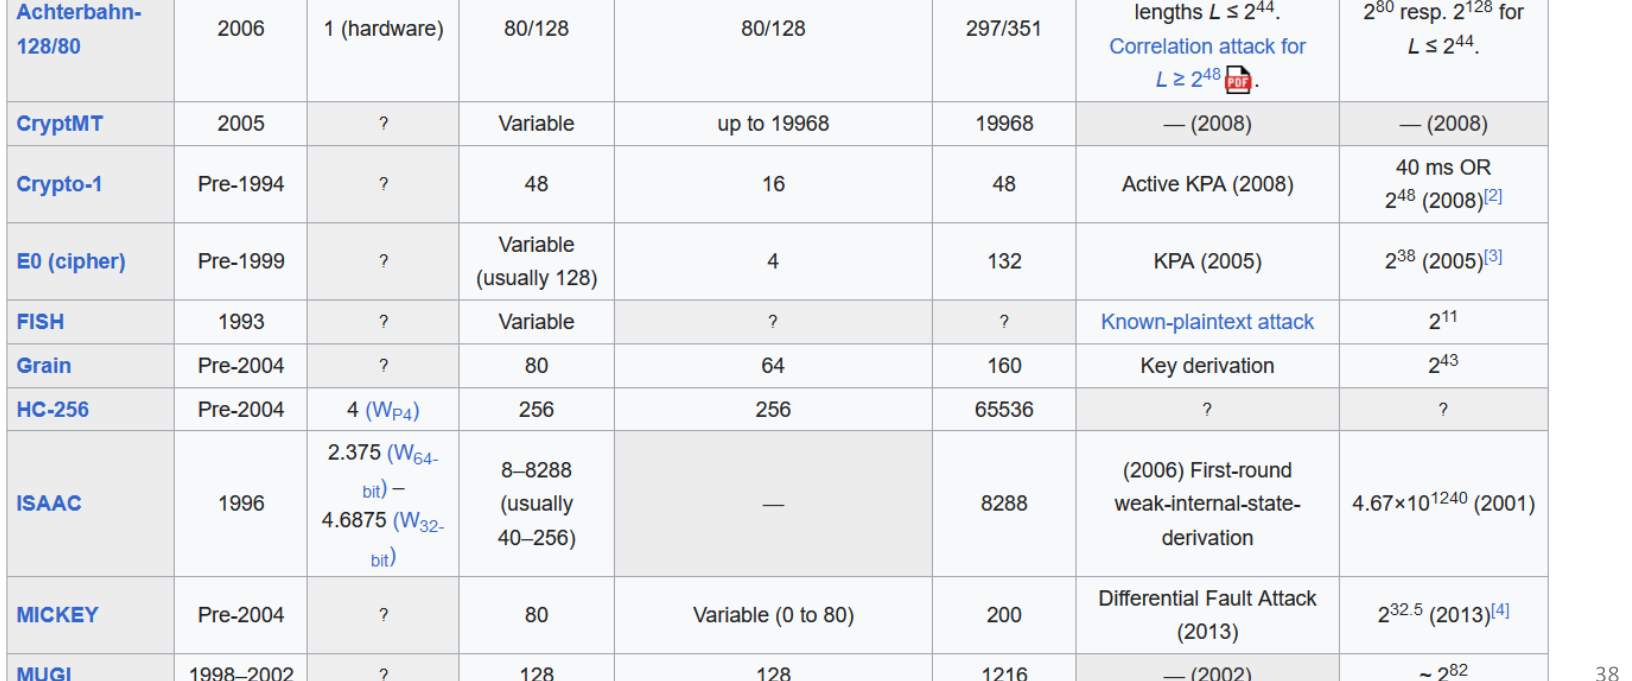
\includegraphics[width=178.50mm,height=187.11mm]{../../images/llm/page_038_img_01.png}%
\end{textblock*}

\end{document}
